\subsection{Rectas}

\begin{postulate}
    Existe al menos una recta.
\end{postulate}

\begin{postulate}
    Toda recta es un conjunto de puntos que contiene al menos dos puntos distintos.
\end{postulate}

\begin{postulate}[\textbf{Postulado de la recta}]
    Si $A$ y $B$ son dos puntos distintos, entonces existe exactamente una recta que los contiene y se denota como $\lne{AB}$.
    
    \begin{figure}[h]
        \centering
        \begin{tikzpicture}[scale=1] 
    \tkzInit[xmax=6,ymax=2, xstep=1]
    
    \tkzDefPoints{% x    y   nombre
                    0  /0   /A,
                    6  /0   /B}
    
    \tkzDrawPoints(A,B)
    \tkzLabelPoints[below](A,B)
    \tkzDrawLine[black,Latex-Latex](A,B)
\end{tikzpicture}
        \caption{La recta $\lne{AB}$}
        \label{fig:plot3}
    \end{figure}
\end{postulate}

\begin{theorem}

Si dos rectas distintas se intersecan, su intersección contiene solamente un punto. Es decir, dos rectas distintas no pueden tener más que un solo punto en común: $l \cap m = \{P\}$.

    \begin{figure}[!h]
        \centering
        \begin{tikzpicture}[scale=1] 
\tkzInit[xmax=6,ymax=2, xstep=1]

\tkzDefPoints{% x    y   name
                0  /0    /A,
                6  /1    /B,
                0  /2    /C,
                6  /0    /D,
                4  /0.67 /P}

\tkzDrawLine[black,Latex-Latex](A,B)
\tkzDrawLine[black,Latex-Latex](C,D)
\tkzLabelLine[style={above right}, pos=1](A,B){$m$}
\tkzLabelLine[style={above right}, pos=-0.1](C,D){$l$}

\tkzDrawPoint(P)
\tkzLabelPoints[above](P)

\end{tikzpicture}
        \caption{$l \cap m = \{P\}$}
        \label{fig:plot19}
    \end{figure}
    
\end{theorem}

\subsection{Plano y Espacio}

\begin{definition}
    Se dice que los puntos de un conjunto son \textit{colineales} si existe una recta que los contiene a todos, de lo contrario se les llama \textit{no colineales}.
\end{definition}

\begin{postulate}
    Todo plano es un conjunto de puntos que contiene, al menos, tres puntos no colineales.
\end{postulate}

\begin{postulate}
    Si \pt{A, B} y \pt{C} son tres puntos no colineales, entonces existe solo un plano que los contiene a todos.
    
    \begin{figure}[!h]
        \centering
        \begin{tikzpicture}[scale=1] 
    \tkzDefPoints{0/0/W,4/0/X,5/2/Y} 
    \tkzDefParallelogram(W,X,Y)
    
    \tkzGetPoint{Z}
    \tkzDrawPolygon(W,X,Y,Z)
    
    \tkzDefPoints{% x    y    nombre
                    1    /1    /A,
                    2.5  /1.5  /B,
                    3.5  /.5   /C,
                    4.2  /1.9  /P}
    
    \tkzDrawPoints(A,B,C)
    \tkzLabelPoint[below](A){$A$}
    \tkzLabelPoint[right](B){$B$}
    \tkzLabelPoint[right](C){$C$}
    
    \tkzLabelPoint[below right](P){$\pi$}
\end{tikzpicture}
        \caption{Plano $\pi$}
        \label{fig:plot5}
    \end{figure}
\end{postulate}

\clearpage

\begin{postulate}
    Si dos puntos de una recta están en un plano, todos los puntos de la recta están en el plano. Simbólicamente si $\pt{A} \in \pi, \pt{B} \in \pi \imply \lne{AB} \in \pi$.
    
    \begin{figure}[!h]
        \centering
        \begin{tikzpicture}[scale=1] 

\tkzDefPoints{0/0/W,4/0/X,5/2/Y} 
\tkzDefParallelogram(W,X,Y)

\tkzGetPoint{Z}
\tkzDrawPolygon(W,X,Y,Z)

\tkzDefPoints{% x     y     name                
                1.2  /.7    /A,
                3.7  /1.1   /B,
                4.2  /1.9   /P}

\tkzDrawPoints(A,B)
\tkzDrawLine[black,Latex-Latex](A,B)
\tkzLabelPoints[below](A,B)
\tkzLabelPoint[below right](P){$\pi$}

\end{tikzpicture}
        \caption{si $\pt{A} \in \pi, \pt{B} \in \pi \imply \lne{AB} \in \pi$}
        \label{fig:plot8}
    \end{figure}
    
\end{postulate}

\begin{definition}
    Se dice que los puntos de un plano son \textit{coplanares} si existe una plano que los contiene a todos, de lo contrario se les llama \textit{no coplanares}.
\end{definition}

\begin{postulate}
    Para todo plano existe un punto $E$ tal que $E$ no está en el plano.
    
    \begin{figure}[!h]
        \centering
        \begin{tikzpicture}[scale=1] 

\tkzDefPoints{0/0/W,4/0/X,5/2/Y} 
\tkzDefParallelogram(W,X,Y)

\tkzGetPoint{Z}
\tkzDrawPolygon(W,X,Y,Z)

\tkzDefPoints{% x    y    name                
                2  /3      /E,
                4.2  /1.9  /P}

\tkzDrawPoints(E)
\tkzLabelPoint[right](E){$E$}
\tkzLabelPoint[below right](P){$\pi$}


\end{tikzpicture}
        \caption{Punto $E$ fuera del plano $\pi$}
        \label{fig:plot7}
    \end{figure}
\end{postulate}

\begin{postulate}
    Si dos planos tiene un punto en común también tiene una recta en común.
    
    \begin{figure}[!h]
        \centering
        \begin{tikzpicture}[scale=1] 

\tkzDefPoints{
%   X   Y     NAME  
    0   /0    /A,
    1   /2    /B,
    2   /2    /C,
    6   /0    /D,
    7   /2    /E,
    2   /3    /F,
    5   /3    /G,
    5   /2    /H,
    2   /0    /I,
    2   /-1   /J,
    5   /0    /K,
    5   /-1   /L,
    0   /1    /M,
    7   /1    /N,
    2   /1    /O,
    3.5 /1    /P,
    5   /1    /Q,
    6   /1.8  /S} 

\tkzDrawPoint(P)
\tkzLabelPoint(P){$P$}
\tkzLabelPoint[below right](S){$\sigma$}

\tkzDrawSegment(A,B)
\tkzDrawSegment(B,C)
\tkzDrawSegment(A,D)
\tkzDrawSegment(D,E)
\tkzDrawSegment(C,F)
\tkzDrawSegment(F,G)
\tkzDrawSegment(G,H)
\tkzDrawSegment(H,E)
\tkzDrawSegment(I,J)
\tkzDrawSegment(K,L)
\tkzDrawSegment(J,L)

\tkzDrawSegment(C,O)
\tkzDrawSegment(H,Q)

\tkzDrawSegment[dashed,lightgray](C,H)
\tkzDrawSegment[dashed,lightgray](I,O)
\tkzDrawSegment[dashed,lightgray](K,Q)

\tkzDrawLine[black,Latex-Latex](M,N)
\tkzLabelLine[style={below}, pos=1](M,N){$l$}

\end{tikzpicture}
        \caption{Punto y recta en común}
        \label{fig:plot9}
    \end{figure}
    
\end{postulate}

\clearpage

\begin{postulate}
    Así como un punto sobre una recta la separa en dos semirectas, también una recta separa a un plano en dos semiplanos y un plano separa el espacio en dos semiespacios.
    
    \begin{figure}[!h]
        \centering
        \begin{tikzpicture}[scale=1] 

\tkzDefPoints{0/0/W,4/0/X,5/2/Y} 
\tkzDefParallelogram(W,X,Y)

\tkzGetPoint{Z}
\tkzDrawPolygon(W,X,Y,Z)

\tkzDefPoints{% x     y     name                
                2    /0     /A,
                3    /2     /B,
                4.2  /1.9   /P,
                1    /0.5   /H1,
                3    /0.5   /H2}


\tkzDrawLine[black,Latex-Latex](A,B)
\tkzLabelLine[style={above left}, pos=1](A,B){$l$}

\tkzLabelPoint[below right](P){$\pi$}
\tkzLabelPoint[below](H1){\scriptsize{$H1$}}
\tkzLabelPoint[below](H2){\scriptsize{$H2$}}

\end{tikzpicture}
        \caption{Separación en semiplanos}
        \label{fig:plot16}
    \end{figure}
\end{postulate}

\begin{postulate}
    Si se tiene un plano $\pi$, una recta $m$ en el plano y un segmento $\seg{AB}$ cuyos extremos, los puntos $A$ y $B$, están en los dos semiplanos que determina $m$ en $\pi$, entonces el segmento $\seg{AB}$ interseca a la recta $m$.
    
    \begin{figure}[!h]
        \centering
        \begin{tikzpicture}[scale=1] 
    \tkzDefPoints{0/0/W,4/0/X,5/2/Y} 
    \tkzDefParallelogram(W,X,Y)
    
    \tkzGetPoint{Z}
    \tkzDrawPolygon(W,X,Y,Z)
    
    \tkzDefPoints{% x     y     nombre                
                    2    /0     /A,
                    3    /2     /B,
                    4.2  /1.9   /P,
                    1    /0.5   /H1,
                    3    /0.5   /H2,
                    1.5  /1.5   /R,
                    3.8  /0.8   /S}
    
    \tkzDrawPoints(R,S)
    \tkzLabelPoint[below](R){$A$}
    \tkzLabelPoint[below](S){$B$}
    \tkzDrawSegment(R,S)
    
    \tkzDrawLine[black,Latex-Latex](A,B)
    \tkzLabelLine[style={below right}, pos=1](A,B){$m$}
    
    \tkzLabelPoint[below right](P){$\pi$}
    \tkzLabelPoint[below](H1){\scriptsize{$H1$}}
    \tkzLabelPoint[below](H2){\scriptsize{$H2$}}
\end{tikzpicture}
        \caption{Segmento interseca a la recta}
        \label{fig:plot17}
    \end{figure}

    Dicho de otra manera, dada una recta $m$ y un plano $\pi$ que la contiene, los puntos de plano que no están en $m$ forman dos conjuntos tales que:

    \begin{itemize}
        \item Cada uno de los conjuntos del plano es un conjunto convexo.
        \item Si un punto $A$ está en uno de los conjuntos, y un punto $B$ está en el otro, entonces el segmento $\seg{AB}$ interseca a la recta $m$.
    \end{itemize}
    
\end{postulate}

\begin{theorem}
    Dada una recta $m$ y un punto $A$ tal que $A \not \in m$, existe un plano que contiene a $A$ y $m$ y ese plano es único.
 
    \begin{figure}[!h]
        \centering
        \begin{tikzpicture}[scale=0.75]
    % Define the points of the triangle
    \tkzDefPoint(0,0){A}
    \tkzDefPoint(5,0){B}
    \tkzDefPoint(-2,3){C}
    
    % Draw the triangle
    \tkzDrawPolygon(A,B,C)
    %\tkzDrawPoints(A,B,C)

    \tkzLabelPoint[left](A){$A$}
    \tkzLabelPoint[above](C){$B$}
    \tkzLabelPoint[right](B){$C$}
    
    % Draw the central angle
    \tkzMarkAngle[size=1cm](B,A,C)
    \tkzLabelAngle[pos=0.5](B,A,C){$\theta$}
    
    % Draw the ticks on the sides of the included angle
    \tkzMarkSegment[mark=|](A,B)
    \tkzMarkSegment[mark=||](A,C)
\end{tikzpicture}
        \caption{Plano único que contiene a $A$ y $m$}
        \label{fig:plot23}
    \end{figure}
        
\end{theorem}

\clearpage

\begin{definition}[\textbf{Rectas Coplanares}]
Dos o más rectas en un mismo plano se denominan coplanares.

    \begin{figure}[!h]
        \centering
        
\begin{tikzpicture}[scale=0.8]
    
    % Define los puntos del triángulo
    \tkzDefPoint(0,0){A}
    \tkzDefPoint(5,0){B}
    \tkzDefPoint(3,3){C}
    
    % Dibuja el triángulo
    \tkzDrawPolygon(A,B,C)

    %\tkzDrawPoints(A,B,C)
    \tkzLabelPoint[left](A){$A$}
    \tkzLabelPoint[right](B){$B$}
    \tkzLabelPoint[above](C){$C$}
    
    % Marca cada lado con barritas
    \tkzMarkSegment[mark=|](A,B)
    \tkzMarkSegment[mark=||](B,C)
    \tkzMarkSegment[mark=|||](A,C)
\end{tikzpicture}
        \caption{Rectas coplanares}
        \label{fig:plot27}
    \end{figure}
    
\end{definition}

\begin{definition}[\textbf{Rectas paralelas}]
Dos o más rectas coplanares que no se intersecan se denominan \textit{paralelas}.

    \begin{figure}[!h]
        \centering
        \begin{tikzpicture}[scale=0.8,rotate=237]
    
    % Define los puntos de un triángulo
    \tkzDefPoint(0,0){A}
    \tkzDefPoint(5,0){B}
    \tkzDefPoint(3,3){C}
    
    % Dibuja el triángulo
    \tkzDrawPolygon(A,B,C)

    %\tkzDrawPoints(A,B,C)
    \tkzLabelPoint[above](A){$D$}
    \tkzLabelPoint[left](B){$E$}
    \tkzLabelPoint[right](C){$F$}
    
    % Marca cada lado con barritas
    \tkzMarkSegment[mark=|](A,B)
    \tkzMarkSegment[mark=||](B,C)
    \tkzMarkSegment[mark=|||](A,C)
\end{tikzpicture}
        \caption{Rectas paralelas}
        \label{fig:plot28}
    \end{figure}
    
\end{definition}

\begin{definition}[\textbf{Rectas concurrentes}]
Dos o mas rectas coplanares que se intersecan en un mismo punto se denominan \textit{concurrentes}.

    \begin{figure}[!h]
        \centering
        
\begin{tikzpicture}[scale=0.8]
    % Define the points of the triangle
    \tkzDefPoint(0,0){A}
    \tkzDefPoint(5,0){B}
    \tkzDefPoint(3,3){C}
    
    % Draw the triangle
    \tkzDrawPolygon(A,B,C)

    %\tkzDrawPoints(A,B,C)
    \tkzLabelPoint[left](A){$A$}
    \tkzLabelPoint[right](B){$B$}
    \tkzLabelPoint[above](C){$C$}
    
    % Draw the marked angles
    \tkzMarkAngle[size=1cm](B,A,C)
    %\tkzLabelAngle[pos = 0.7](B,A,C){$\alpha$}
    \tkzMarkAngle[size=1cm](C,B,A)
    \tkzMarkAngle[size=1.1cm](C,B,A)
    %\tkzLabelAngle[pos = 0.7](C,B,A){$\beta$}
    
    % Mark the non-included side with ticks
    \tkzMarkSegment[mark=||](A,C)
\end{tikzpicture}
        \caption{Rectas concurrentes}
        \label{fig:plot29}
    \end{figure}

\end{definition}

\clearpage

\begin{postulate}
    Dada una recta $m$ existe al menos un punto $P$ que no pertenece a $m$.
    
    \begin{figure}[h]
        \centering
        \begin{tikzpicture}[scale=1] 
    \tkzInit[xmax=6,ymax=2, xstep=1]
    
    \tkzDefPoints{% x    y   nombre
                    0  /0   /A,
                    6  /0   /B,
                    2  /1   /P}
    
    \tkzDrawPoint(P)
    \tkzLabelPoint[right](P){$P$}
    \tkzDrawLine[black,Latex-Latex](A,B)
    \tkzLabelLine[style={above}, pos=1](A,B){$m$}
\end{tikzpicture}
        \caption{$P \notin m$}
        \label{fig:plot2}
    \end{figure}
\end{postulate}

\begin{postulate}[\textbf{Rectas paralelas}]
    Por un punto exterior a una recta dada se puede trazar una recta única que sea paralela a ella. Dos rectas $l$ y $m$ son paralelas si están en un mismo plano y su intersección es vacía: $l \cap m = \emptyset$.
    
    \begin{figure}[!h]
        \centering
        \begin{tikzpicture}[scale=1] 
\tkzInit[xmax=6,ymax=2, xstep=1]

\tkzDefPoints{% x    y   name
                0  /0   /A,
                6  /1   /B,
                0  /1   /C,
                6  /2   /D,
                3  /1.5 /P}

\tkzDrawLine[black,Latex-Latex](A,B)
\tkzDrawLine[black,Latex-Latex](C,D)
\tkzLabelLine[style={above right}, pos=1](A,B){$m$}
\tkzLabelLine[style={above right}, pos=1](C,D){$l$}

\tkzDrawPoint(P)
\tkzLabelPoints[above](P)

\end{tikzpicture}
        \caption{Rectas paralelas: $l \cap m = \emptyset$}
        \label{fig:plot15}
    \end{figure}

\end{postulate}

\begin{definition}[\textbf{Espacio}]
    El espacio es el conjunto de todos los puntos.
\end{definition}

\begin{postulate}
    El espacio contiene, al menos, cuatro puntos no coplanares.
\end{postulate}

\begin{postulate}
    En el espacio, si se tiene un plano y un segmento con extremos en los dos semiplanos, el segmento interseca al plano.
\end{postulate}

\begin{definition}[\textbf{Conjunto convexo}]
    Un conjunto $A$ se llama \textit{convexo} si para cada par de puntos $\pt{R}$ y $\pt{S}$, que pertenecen a él, el segmento $\seg{RS}$ está contenido en $A$.

    \begin{figure}[h!]

        \centering

        \begin{subfigure}[b]{.5\textwidth}
            \centering
            \begin{tikzpicture}[scale=0.75,rotate=203]
    % Define the points of the triangle
    \tkzDefPoint(0,0){A}
    \tkzDefPoint(5,0){B}
    \tkzDefPoint(-2,3){C}
    
    % Draw the triangle
    \tkzDrawPolygon(A,B,C)
    %\tkzDrawPoints(A,B,C)

    \tkzLabelPoint[above](A){$D$}
    \tkzLabelPoint[right](C){$E$}
    \tkzLabelPoint[left](B){$F$}
    
    % Draw the central angle
    \tkzMarkAngle[size=1cm](B,A,C)
    \tkzLabelAngle[pos=0.5](B,A,C){$\theta$}
    
    % Draw the ticks on the sides of the included angle
    \tkzMarkSegment[mark=|](A,B)
    \tkzMarkSegment[mark=||](A,C)
\end{tikzpicture}
            \label{fig:plot24}
            \caption{Convexo}            
        \end{subfigure}%
        \begin{subfigure}[b]{.5\textwidth}
            \centering
            \begin{tikzpicture}[scale=0.8]

    % Define puntos del triángulo
    \tkzDefPoint(0,0){A}
    \tkzDefPoint(5,0){B}
    \tkzDefPoint(1,3){C}
    
    % Dibuja el triángulo
    \tkzDrawPolygon(A,B,C)

    %\tkzDrawPoints(A,B,C)
    \tkzLabelPoint[left](A){$A$}
    \tkzLabelPoint[right](B){$B$}
    \tkzLabelPoint[above](C){$C$}
        
    % Dibuja los ángulos marcados
    \tkzMarkAngle[size=1cm](B,A,C)
    \tkzLabelAngle[pos=0.6](B,A,C){$1$}
    \tkzMarkAngle[size=1.1cm](C,B,A)
    \tkzLabelAngle[pos=0.7](C,B,A){$2$}
    
    % Dibuja las barrita en los lados del ángulo incluído.
    \tkzMarkSegment[mark=|](A,B)
    
    % Rellena la región de los ángulos marcados
    %\tkzFillAngle[fill= gray!40, opacity=.2](B,A,C)
    %\tkzFillAngle[fill= gray!40, opacity=.2](C,B,A)
    
\end{tikzpicture}

            \label{fig:plot25}
            \caption{No Convexo}            
        \end{subfigure}
        
        \centering
        \caption{Convexidad}
        \label{fig:convexidad}
    
    \end{figure}
    
\end{definition}

\clearpage

\begin{postulate}[\textbf{Postulado de separación del plano}]
    Dada una recta $m$ y un plano que la contiene, los puntos del plano que no están en $m$ forman dos conjuntos:

    \begin{itemize}
        \item Cada uno de los conjuntos del plano es un conjunto convexo.
        \item Si un punto $\pt{R}$ está en uno de los conjuntos y un punto $\pt{S}$ está en el otro, entonces el segmentos $\seg{RS}$ interseca a la recta $m$.
    \end{itemize}
\end{postulate}

\begin{definition}[\textbf{Arista}]
    Una recta en el plano que determina dos conjuntos convexos llamados semiplanos se denomina \textit{arista} o \textit{borde} de cada uno de ellos.

    \begin{figure}[!h]
        \centering
        \begin{tikzpicture}[scale=0.8,rotate=215]
    
    % Define los puntos del triángulo
    \tkzDefPoint(0,0){A}
    \tkzDefPoint(5,0){B}
    \tkzDefPoint(1,3){C}
    
    % Dibuja el triángulo
    \tkzDrawPolygon(A,B,C)

    %\tkzDrawPoints(A,B,C)
    \tkzLabelPoint[above](A){$D$}
    \tkzLabelPoint[left](B){$E$}
    \tkzLabelPoint[right](C){$F$}
        
    % Dibuja los ángulos marcados
    \tkzMarkAngle[size=1cm](B,A,C)
    \tkzLabelAngle[pos=0.6](B,A,C){$1$}
    \tkzMarkAngle[size=1.1cm](C,B,A)
    \tkzLabelAngle[pos=0.7](C,B,A){$2$}
    
    % Dibuja las barritas de del ángulo incluídos
    \tkzMarkSegment[mark=|](A,B)
    
    % Rellena la región de los ángulos marcados.
    %\tkzFillAngle[fill= gray!40, opacity=.2](B,A,C)
    %\tkzFillAngle[fill= gray!40, opacity=.2](C,B,A)
    
\end{tikzpicture}

        \caption{Arista}
        \label{fig:plot26}
    \end{figure}
    
\end{definition}

\begin{postulate}[\textbf{Separación del espacio}]
    Los puntos del espacio que no están en un plano dado forman dos conjuntos denominados semiespacios tales que:

    \begin{itemize}
        \item Los dos conjuntos, uno a cada lado del plano, son convexos.
        \item Si un punto $\pt{R}$ está en uno de los conjuntos y un punto $\pt{S}$ está en el otro, entonces el segmentos $\seg{RS}$ interseca al plano en un punto.
    \end{itemize}
\end{postulate}

\subsection{Coordenadas y Distancia}

\begin{postulate}
    El conjunto de puntos de una recta y el conjunto de números reales se coinciden uno a uno.
\end{postulate}

\begin{definition}
    A la correspondencia entre los puntos de una recta y los números reales se le conoce como un \textit{sistema de coordenadas}. Se llama \textit{coordenada} al número real asociado a un punto dado. Al punto con la coordenada cero se le conoce como \textit{origen}.
\end{definition}

\begin{postulate}[\textbf{Postulado de la regla}]
    Toda recta tiene un sistema de coordenadas. 
\end{postulate}

Suponiendo que $\overleftrightarrow{l}$ es un recta con un sistema de coordenadas $c$, si $P \in \overleftrightarrow{l}$, y la coordenada de $P$ es $x$, entonces esto se denota como $c(P) = x$.

\clearpage

\begin{postulate}[\textbf{Postulado de ubicación de la regla}]

    Sea $\overleftrightarrow{l}$ una recta tal que $P \in \overleftrightarrow{l}$ y  $Q \in \overleftrightarrow{l}$, donde $P \neq Q$. Entonces existe un sistema de coordenadas $c$ para $\overleftrightarrow{l}$ tal que $c(P)=0$ y $c(Q)$ es un número positivo.

    \begin{figure}[!h]
        \centering
        \begin{tikzpicture}[scale=0.8] 
    \tkzInit[xmax=5,ymax=0] 
    \tkzDrawX[label={}]
    \tkzDefPoints{0/0/FA,3/0/FP,0/1/A,3/1/P,5/1/B}
    
    \tkzDrawPoints(FA,FP,A,P)
    \tkzLabelPoint[above](A){$P$}
    \tkzLabelPoint[above](P){$Q$}
    \tkzDrawLine[black,Latex-Latex](A,B)
    \tkzLabelLine[above right,pos=1](A,B){$l$}
    \tkzLabelPoint[above](FA){$c(P)$}
    \tkzLabelPoint[above](FP){$c(Q)$}
    \tkzLabelPoint[below](FA){$0$}
    \tkzLabelPoint[below](FP){$x$}
\end{tikzpicture}
        \caption{Sistema de coordenadas}
        \label{fig:plot4}
    \end{figure}

\end{postulate}

\begin{definition}
    Sea $\overleftrightarrow{l}$ una recta con un sistema de coordenadas $c$, tal que si $P \in \overleftrightarrow{l}$ y $Q \in \overleftrightarrow{l}$ y $c(P) = x$ y $c(Q) = y$, entones \textit{la distancia} de $P$ a $Q$, denotada como $PQ$, se define como: $$PQ = |y - x|$$.

    Es decir, \textit{la distancia} entre dos puntos dados es el valor absoluto de la diferencia de sus coordenadas.
\end{definition}

\begin{postulate}[\textbf{Postulado de la distancia}]
A cada par de puntos de un plano les corresponde un único número real mayor o igual que 0, conocido como la distancia.
\end{postulate}

\begin{postulate}
Si se tienen dos puntos $A$ y $B$, $A = B$, si y solamente si $AB = 0$.
Si se tienen dos puntos $C$ y $D$, entonces $CD = DC$
\end{postulate}

\begin{theorem}
    Si se tienen tres puntos $F,G$ y $H$, entonces $FG + GH \ge FH$. En caso de que $F,G$ y $H$ no sean colineales se cumple que $FG + GH > FH$.

    \begin{corolary}
    La distancia más corta entre dos puntos es una línea recta.
    \end{corolary}
    
\end{theorem}

\begin{definition}[\textbf{Estar entre}]
    Sea $\overleftrightarrow{l}$ una recta, y $A, B$ y $C$ tres puntos distintos en ella. Se dice que $B$ \textit{está entre} $A$ y $C$, denotado como $A-B-C$ si y solo sí se cumple una de las siguientes condiciones:

    \begin{equation}
            AB + BC = AC \\
    \end{equation}
    \begin{equation}
        c(A) < c(B) < c(C)
    \end{equation}
    \begin{equation}
        c(A) > c(B) > c(C)
    \end{equation}

    \begin{figure}[!h]
        \centering
        \begin{tikzpicture}[scale=1] 
    \tkzInit[xmax=6,ymax=2, xstep=1]
    
    \tkzDefPoints{% x    y   nombre
                    0  /0   /A,
                    3  /0   /B,
                    6  /0   /C}
    
    \tkzDrawPoints(A,B,C)
    \tkzLabelPoints[below](A,B,C)
    \tkzDrawLine[black,Latex-Latex](A,C)
\end{tikzpicture}
        \caption{$B$ entre $A$ y $C$}
        \label{fig:plot10}
    \end{figure}
    
\end{definition}

\clearpage

\begin{theorem}
    Si $A$ y $C$ son dos puntos distintos, entonces existe un punto $B$ tal que $A-B-C$.
\end{theorem}

\begin{theorem}
    Si $A$ y $B$ son dos puntos distintos, entonces existe un punto $C$ tal que $B$ esté entre $A$ y $C$.
\end{theorem}

\begin{postulate}
    Dados tres puntos colineales distintos, uno y solo uno está entre los otros dos.
    
    \begin{figure}[!h]
        \centering
        \begin{tikzpicture}[scale=1] 
    \tkzInit[xmax=6,ymax=2, xstep=1]
    
    \tkzDefPoints{% x    y   nombre
                    0  /0   /A,
                    1  /0   /B,
                    2  /0   /C,
                    4  /0   /D,
                    5  /0   /E,
                    6  /0   /F,
                    8  /0   /G,
                    9  /0   /H,
                    10 /0   /I}
    
    \tkzDrawPoints(A,B,C,D,E,F,G,H,I)
    \tkzLabelPoints[below](A,B,C)
    
    \tkzLabelPoint[below](D){$A$}
    \tkzLabelPoint[below](E){$C$}
    \tkzLabelPoint[below](F){$B$}
    
    
    \tkzLabelPoint[below](G){$C$}
    \tkzLabelPoint[below](H){$A$}
    \tkzLabelPoint[below](I){$B$}
    
    
    \tkzDrawLine[black,Latex-Latex](A,C)
    \tkzDrawLine[black,Latex-Latex](D,F)
    \tkzDrawLine[black,Latex-Latex](G,I)
\end{tikzpicture}
        \caption{Entre dos puntos}
        \label{fig:plot12}
    \end{figure}
    
\end{postulate}

\begin{definition}[\textbf{Segmento}]
    Sea $\lne{AB}$ una recta. La unión de $A$ y $B$ con el conjunto de todos los puntos entre $A$ y $B$ se conoce como \textit{segmento} y se denota $\seg{AB}$. A los puntos $A$ y $B$ se los denomina los \textit{extremos} del segmento, y el resto de los puntos se denominan \textit{puntos interiores} del segmento. 
\end{definition}

\begin{definition}[\textbf{Distancia}]
    Sea $\seg{AB}$ un segmento, entonces la longitud del segmento $\seg{AB}$ se define como la distancia entre $A$ y $B$, denotada como $AB$.
\end{definition}

\begin{postulate}
La distancia más corta entre dos puntos es el segmento que los une.
\end{postulate}

\begin{definition}[\textbf{Segmento congruente}]
    Dados dos segmentos $\seg{AB}$ y $\seg{CD}$, se dice que son \textit{congruentes} si $AB = CD$, y se denota  como $\seg{AB} \cong \seg{CD}$.
\end{definition}

\begin{theorem}
    La congruencia de segmentos es reflexiva: dado el segmento $\seg{AB}$, entonces $\seg{AB} \cong \seg{AB}$.
\end{theorem}

\begin{theorem}
    La congruencia de segmentos es simétrica: si $\seg{AB} \cong \seg{CD}$, entonces $\seg{CD} \cong \seg{AB}$.
\end{theorem}

\begin{theorem}
    La congruencia de segmentos es transitiva: si $\seg{AB} \cong \seg{CD}$ y $\seg{CD} \cong \seg{EF}$, entonces $\seg{AB} \cong \seg{EF}$.
\end{theorem}

\begin{theorem}[\textbf{Teorema de suma de segmentos}]
    Si $A-B-C$, $R-S-T$, $\seg{AB} \cong \seg{RS}$ y $\seg{BC} \cong \seg{ST}$, entonces $\seg{AC} \cong \seg{RT}$.
\end{theorem}

\begin{theorem}[\textbf{Teorema de resta de segmentos}]
    Si $A-B-C$, $R-S-T$, $\seg{AB} \cong \seg{RS}$ y $\seg{AC} \cong \seg{RT}$, entonces $\seg{BC} \cong \seg{ST}$.
\end{theorem}

\begin{theorem}[\textbf{Teorema de bisección de segmentos}]
    Si $\seg{AC} \cong \seg{RT}$, $\pt{B}$ el punto medio de $\seg{AC}$, $\pt{S}$ el punto medio de $\seg{RT}$, entonces $\seg{AB} \cong \seg{RS}$.
\end{theorem}

\begin{definition}[\textbf{Rayo}]
    Sea $\lne{AB}$ una recta. El rayo $AB$, denotado como $\ray{AB}$ es el conjunto de todos los puntos $C$, tal que $C \in \lne{AB}$ y además $A$ no está entre $B$ y $C$. El punto $A$ se conoce como el \textit{extremo} del rayo, y el resto de los puntos se denominan \textit{puntos interiores}.
\end{definition}

\clearpage

\begin{definition}[\textbf{Rayos opuestos}]
    Sea $\lne{AC}$ una recta. Si $A-B-C$, entonces $\ray{BA}$ y $\ray{BC}$ denominan \textit{rayos opuestos}.

    \begin{figure}[h]
        \centering
        \begin{tikzpicture}[scale=1] 
    \tkzInit[xmax=6,ymax=2, xstep=1]
    
    \tkzDefPoints{% x    y   nombre
                    0  /0   /A,
                    6  /0   /B}
    
    \tkzDrawLine[black,Latex-Latex](A,B)
    \tkzLabelLine[style={above}, pos=1](A,B){$l$}
\end{tikzpicture}
        \caption{Rayos opuestos}
        \label{fig:plot1}
    \end{figure}
\end{definition}

\begin{postulate}[\textbf{Postulado de trazado de puntos}]
    Dados un rayo $\ray{AB}$ y un número real $r$, tal que $r > 0$. Entonces existe exactamente un punto $C$, tal que $C \in \ray{AB}$ y $AC = r$.

    \begin{figure}[h]
        \centering
        
\begin{tikzpicture}[scale=0.8] 
    \tkzInit[xmax=6,ymax=0] 
    \tkzDrawX[label={}]
    \tkzDefPoints{
        0 /0 /CA,
        3 /0 /CB,
        6 /0 /CC,
        0 /0 /A,
        3 /0 /B,
        6 /0 /C}
    
    \tkzDrawPoints(A,B,C,CA,CB,CC)
    
    \tkzLabelPoint[above](A){$A$}
    \tkzLabelPoint[above](B){$B$}
    \tkzLabelPoint[above](C){$C$}
    
    %\tkzDrawSegment[add=0.0 and 0.3, -Latex](A,C)
    
    \tkzLabelPoint[below](CA){$0$}
    \tkzLabelPoint[below](CC){$r$}
\end{tikzpicture}
        \caption{$C \in \ray{AB}$ y $AC = r$}
        \label{fig:plot18}
    \end{figure}
    
\end{postulate}

\begin{definition}[\textbf{Punto medio}]
    Sea $A-B-C$. Se dice que $B$ es el \textit{punto medio} de $\seg{AC}$ si y solo si $AB = BC$. En ese caso se dice que $B$ biseca a $\seg{AC}$.

    En general, cuando un conjunto cualquiera $S$ donde $S \cap \seg{AC} = \{B\}$, se dice que $S$ biseca a $\seg{AC}$.
\end{definition}

\begin{theorem}[\textbf{Teorema del punto medio}]
    Cada segmento tiene un único punto medio.
\end{theorem}

\begin{theorem}
    Sea $M$ el punto medio de $\seg{AB}$, donde $c(A) = a$, $c(M) = m$ y $c(B) = b$, entonces se cumple que $m = \dfrac{a +b }{2}$.

    \begin{figure}[h]
        \centering
        \begin{tikzpicture}[scale=1] 

\tkzDefPoints{0/0/W,4/0/X,5/2/Y} 
\tkzDefParallelogram(W,X,Y)

\tkzGetPoint{Z}
\tkzDrawPolygon(W,X,Y,Z)

\tkzDefPoints{% x    y    name
                1    /1    /A,
                2.5  /1.5  /B,
                3.5  /.5   /C,
                4.2  /1.9  /P}

\tkzDrawPoints(A,B,C)
\tkzLabelPoint[below](A){$E$}
\tkzLabelPoint[right](B){$D$}
\tkzLabelPoint[right](C){$F$}

\tkzLabelPoint[below right](P){$\sigma$}


\end{tikzpicture}
        \caption{Punto medio}
        \label{fig:plot6}
    \end{figure}
    

    Hay que considerar que si $M$ es el punto medio de $\seg{AB}$, entonces $AM = MB$, y $a < b$, por lo tanto se puede demostrar que:

    \begin{equation*}
        \begin{split}
            m - a &= b - m \\
            2m &= a + b \\
            m &= \dfrac{a + b}{2}
        \end{split}
    \end{equation*}
\end{theorem}

\clearpage

\begin{theorem}[\textbf{Teorema de construcción del segmento}]
    Dado un segmento $\seg{AB}$ y un rayo $\ray{CD}$, hay exactamente un punto $\pt{E}$, con $\pt{E} \in \ray{CD}$, tal que $\seg{AB} \cong \seg{CE}$.   

    \begin{figure}[h]
        \centering
        \begin{tikzpicture}[scale=1] 
    \tkzInit[xmax=6,ymax=2, xstep=1]
    
    \tkzDefPoints{% x    y   nombre
                    0  /0   /A,
                    3  /0   /B,
                    6  /0   /C}
    
    \tkzDrawPoints(A,B,C)
    \tkzLabelPoints[below](A,B,C)
    \tkzDrawLine[black,Latex-Latex](A,C)
\end{tikzpicture}
        \caption{Construcción del segmento}
        \label{fig:plot10}
    \end{figure}
    
\end{theorem}

\subsection{Propiedades del Conjunto de los Números Reales}

Las siguientes propiedades se cumplen para todos los elementos $a,b,c,d$ del conjunto de los números reales. Estas leyes resultan convenientes en el desarrollo de demostraciones.

\vspace{0.5em}

\begin{center}
    \begin{tabular}{ll}
        \textit{Ley de reflexividad} & $a = a$ \\
        \textit{Ley de simetría} & Si $a = b$ entonces $b = a$ \\
        \textit{Ley de transitividad} &  Si $a = b$, y $b = c$, entonces $a = c$\\
        \textit{Ley de la suma} & Si $a = b$ y $c = d$, entonces $a + c = b + d$ \\
        \textit{Ley de la multiplicación} & Si $a = b$ y $c = d$, entonces $ac = bd$\\
        \textit{Ley de la división} & Si $a = b$ y $c = d \neq 0$, entonces $\dfrac{a}{c} = \dfrac{b}{d}$\\
    \end{tabular}
    \label{tab:ralnumprops1}
\end{center}

\vspace{0.5em}

\begin{center}
    \begin{tabular}{l m{10em} m{10em}}
        & \textit{Suma} & \textit{Multiplicación} \\
        \hline
        \textit{Ley de clausura} & $a + b$ es un número real para todo $a$ y $b$ & $ab$ es un número real para todo $a$ y $b$ \\
        \textit{Ley asociativa} & Para todo $a,b,c$, $(a+b)+c = a+(b+c)$ & $(ab)c = a(bc)$ \\
        \textit{Elemento identidad} & $a + 0 = a$ & $a \cdot 1 = a$ \\
        \textit{Elemento inverso} & $a + (-a) = 0$ & $a \cdot a^{-1} = 1$
    \end{tabular}
    \label{tab:ralnumprops2}
\end{center}

\vspace{0.5em}

Y vinculando a estas dos operaciones tenemos la \textit{ley distributiva}: $a(b +c) = ab + ac$

\textit{Ley de la sustitución}: si $a$ y $b$ son dos nombres para para el mismo número real, entonces cualquiera puede ser substituido por el otro en cualquier expresión matemática sin alterar la verdad de valor de la expresión.

\begin{center}
    \begin{tabular}{ll}
        \textit{Ley de cancelación de la suma} & si $a + b = a + c$ entonces $b = c$ \\
        \textit{Ley de cancelación de la multiplicación I} & si $ab = ac$ y $a \neq 0$, entonces $b = c$ \\
        \textit{Ley de cancelación de la multiplicación II} & si $\dfrac{ab}{ac} = \dfrac{b}{c}$
    \end{tabular}
    \label{tab:ralnumprops1}
\end{center}


\nocite{MGECED05}
\nocite{MGECED06}
\nocite{MGECED07}

\clearpage



%Bibliografía de esta sección
\printbibliography[heading=subbibliography,title={Bibliografía}]